\documentclass[10pt,a4paper]{book}
\usepackage[utf8]{inputenc}
\usepackage[spanish]{babel}
\usepackage{amsmath}
\usepackage{amsfonts}
\usepackage{amssymb}
\usepackage{makeidx}
\usepackage{graphicx}
\usepackage{color}
\usepackage{fancyvrb}
\usepackage[colorlinks=true,linkcolor=black,urlcolor=black]{hyperref}
\author{Maqueavelo Hidrovo, José Jácome, Erik Quijije}
\title{Proyecto II}
%Comando para hacer un rectangulo en una palabra
\newcommand{\HRule}{\rule{\linewidth}{0.5mm}}

\begin{document}
\begin{titlepage}
\begin{center}

\includegraphics[scale=1]{espe.jpg}\\ 
\vfill
\textsc{\LARGE UNIVERSIDAD DE LAS FUERZAS ARMADAS ESPE}\\[1.5cm] 
\textsc{\Large Proyecto de Matemática Superior}\\[0.5cm] 
% Title
\HRule \\[0.4cm]
{ \huge \bfseries Desarrollo de varias ondas de audio a través de una síntesis de Fourier.
 \\[0.4cm] }

\HRule \\[1.5cm]
\textsc{\Large AUTORES}\\[0.5cm]
\emph{\Large \begin{itemize}
\item Hidrovo Andrés	
\item Jácome José
\item Quijije Erik
\end{itemize}}


\vfill

% Bottom of the page
{\large \today}
\end{center}
\end{titlepage}

\tableofcontents % indice de contenidos
\addcontentsline{toc}{chapter}{Indíce del Proyecto}
\phantomsection
\clearpage


\section{Tema}

Desarrollo de la transformada de Fourier a partir de una onda de audio.\\

\section{Objetivo General}

A partir de una onda de audio obtener la transformada de Fourier y analizar sus características \\

\section{Objetivos Específicos}

Realizar una transformación de Fourier de una onda de Audio.\\
Usar una onda de audio dada la amplitud y el tiempo para obtener una onda en función de la amplitud vs frecuencia.\\
Usar el programa Matlab para generar la representar el Hecho.\\

\section{Marco Teórico}

\subsection{Transformada de Fourier}

Fourier  es una técnica matemática, desarrollada a finales del siglo XVIII por Jean Bautista Fourier y publicada en su libro \textit{Théorie analitique de la chaleur}, y que da cuenta de la complejidad de los sonidos, más allá de las características de intensidad-tono-timbre, dicha investigación demostro que cualquier forma de onda puede descomponerse en la suma de una serie de ondas senoidales individuales, de frecuencia, amplitud y fase individual. \\
La transformada de Fourier se encarga de convertir la función de amplitud vs tiempo en amplitud vs frecuencia

\subsection{El sonido como una transformada de Fourier}

A la hora de analizar el sonido podemos decir que es una vibración del aire tratable como un fenómeno ondulatorio. Los valores cuantitativos que caracterizan una onda son su \textit{amplitud} y \textit{frecuencia} íntimamente relacionados con los valores cualitativos de volumen y tono. Sin embargo esta manera de describir el sonido no podría diferenciar por ejemplo el tono "Do" de un piano del tono "Do" de un violín, es decir, diferenciar el timbre de estos instrumentos. Realmente el sonido creado por un instrumento musical es una \textit{compleja maraña de pequeñas ondas} a lo largo de una onda fundamental y con correspondiente frecuencia fundamental. Esa frecuencia fundamental es la que corresponde al tono del sonido producido por el instrumento. Las frecuencias de las "pequeñas ondas" que viajan a lo largo de la fundamental producen el timbre del sonido.\\

El movimiento de las moléculas de aire debido a los cambios de presión y el retorno a sus posiciones iniciales (elasticidad del medio) tiene la dirección de la perturbación generada, por ello, la onda sonora se denomina longitudinal. Las podemos diferenciar de ondas transversales como las de la vibración de una cuerda.\\

El sonido de una pieza musical, compuesto por una superposición de ondas de los distintos instrumentos según el paso del tiempo se puede analizar mediante la "Transformación de Fourier". Si visualizásemos las ondas de un sonido complejo como una pieza musical, no podríamos reconocer en la superposición final, de qué instrumento procede cada frecuencia. Con esta transformación matemática conseguimos a partir de una señal sonora que varía en el tiempo (frecuencias y amplitudes), representarla como sumas de ondas independientes de distintas frecuencias. Por tanto, obtenemos las frecuencias que conforman el sonido que estamos escuchando.

\subsection{Transformada Rápida de Fourier}

Abreviada como FFT (Fast Fourier Transform) es un eficiente algoritmo que permite calcular la transformada de Fourier Discreta y su inversa. \\ Este algoritmo tine una gran importancia en una amplia variedad de aplicaciones, desde el tratamiento digital de señales y filtrado digital. La FFT se encarga de resolver la Transformada Discreta de Fourier,  

\subsection{Espectro Sonoro de un Sonido Complejo}

El análisis a la Fourier de un sonido lo descompone en todas y cada una de las frecuencias que lo forman, y le asigna a cada frecuencia una intensidad o amplitud específica. Al conjunto de frecuencias amplitudes se le llama el espectro del sonido analizado.
En un sonido nuestra sensación de tono que no está determinada únicamente por la "frecuencia" del sonido, cuando éste es complejo, ya que, sencillamente, un sonido complejo no tiene una sola frecuencia, y ni siquiera bastan para definirlo sus armónicos principales. La sensación de "un" sonido es el resultado de toda una serie de ondulaciones de distintas frecuencias, cuyas importancias relativas cambian rápidamente con el tiempo.\\

\begin{center}
	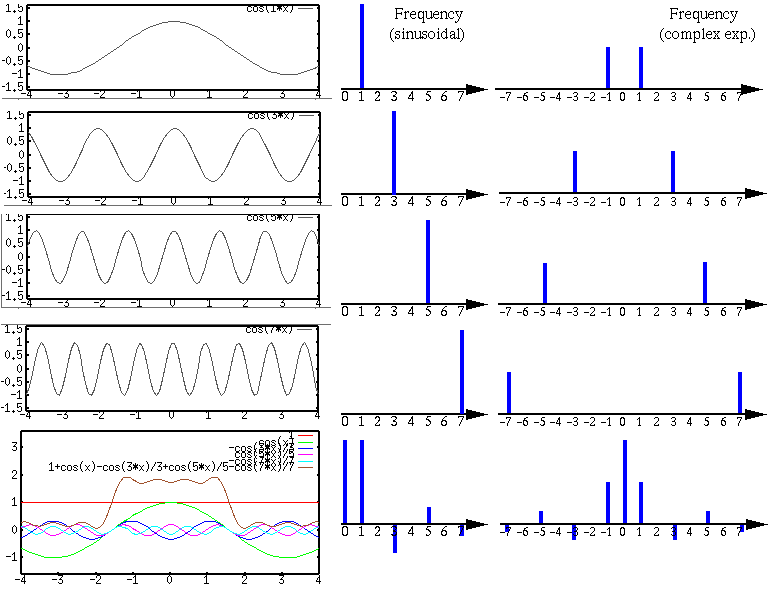
\includegraphics[scale=0.45]{AudioFourier.png}\\
\end{center}

Cualquier forma de onda, a condición de que sea periódica (se repita siempre igual) se puede descomponer en una serie más o menos larga (quizás infinita) de ondas puras (senoidales) llamadas armónicos. Estos armónicos son tales que su combinación o mezcla dan lugar de nuevo al sonido original, y sus frecuencias son múltiplos enteros de la del sonido fundamental.\\

\subsection{Código de Matlab}

\begin{verbatim}
clear;
x=wavread('audiocheck.net_tri_5Hz_-3dBFS_3s.WAV')
%subplot(201)
sound(x)
Y=fft(x);
A=Y.*conj(Y)
f=(100:200);
%subplot(202)
figure
subplot(1,2,1)
plot(x)
subplot(1,2,2)
plot(f,A(1:101));
\end{verbatim}

\subsection{Ejemplo Práctico}

Mediante el programa \textit{Audacity} se puede analizar ondas de audio, así mediante la importación de un archivo de audio en este caso con una Amplitud de 100Hz durante un intervalo de tiempo de 0.010 s entre cada onda, el programa nos da una gráfica idealizada asi:
\begin{center}
	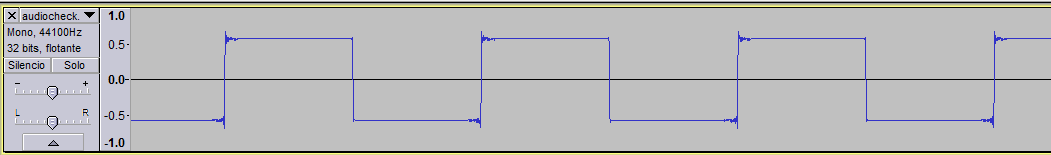
\includegraphics[scale=0.5]{Cuadrada.png} 
\end{center}

Esta gráfica nos muestra una aproximación en Serie de Fourier de la Onda, así el análisis por Transformada de Fourier se empieza con el espectro, que se obtiene al aplicar esta operación:
\begin{center}
	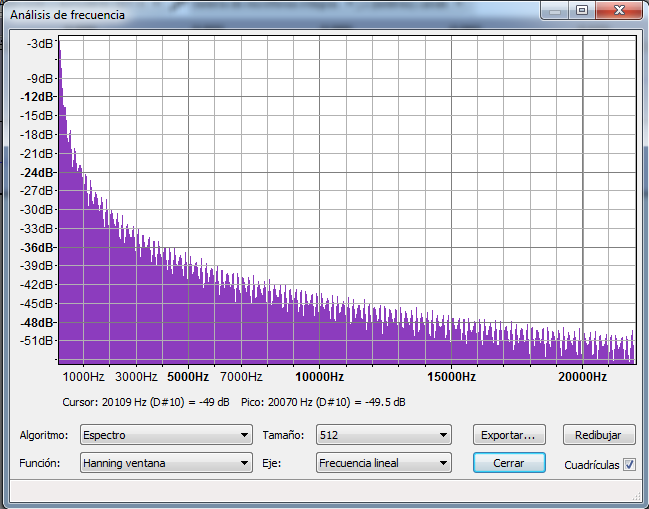
\includegraphics[scale=0.5]{Espectro.png} 
\end{center}

Dicha operación permite manipular la onda de sonido, así reduciendole los bajos o los altos y aplicandole una transformada inversa nos permite obtener una onda de audio " rectificada "\\


\section{Conclusiones}

\begin{itemize}

\item El análisis espectral de señales continuas y no periódicas se puede llevar a cabo usando los métodos de Fourier, con aproximación de una o de varias ondas que forman la onda la onda de sonido.
\item El sonido es una onda periódica en el tiempo que se puede ajustar fácilmente a una serie de Fourier, la transformada de Fourier se usa para poder mejorar el sonido. 
\item Muchos programas básicos de audio como Audacity incorporan los Métodos de Fourier para el análisis de Audio.


\end{itemize}

\section{Recomendaciones}

\begin{enumerate}
\item Realizar los cálculos en un software matemático y el diseño en un programa que permita simular correctamente la onda de sonido con los diferentes parámetros asignados
\item Realizar la simulación del análisis por medio de equipos auditivos y observar de forma gráfica el comportamiento de estas.
\item Tener el equipo necesario para poder llevar a cabo todas las tareas de análisis, ya que al tener falencias no se podrá llegar a comprender de forma clara el trabajo realizado.

\end{enumerate}

\section{Bibliografía}

\begin{enumerate}
\item http://tumblr.charlio.com/post/47242490697/la-transformada-de-fourier-for-dummies
\item http://ensujustamedida.blogspot.com/2011/01/descomponiendo-el-sonido-la.html
\item https://es.wikipedia.org/wiki/
\item http://www.slideshare.net/lichowlin/audacitymanual
\item http://cpms-acusticamusical.blogspot.com/2009/10/analisis-armonico-el-teorema-de-fourier.html
\end{enumerate}

\end{document}